\documentclass[a4paper, 11pt]{article}
\usepackage[slovene]{babel}
\usepackage[utf8]{inputenc}
\usepackage[T1]{fontenc}
\usepackage{amsfonts,amsmath,amssymb}
\usepackage{amsthm}
\usepackage{amsmath}
\usepackage{amssymb}
\usepackage{tikz}
\usepackage{graphicx}
\usepackage{float}
\usepackage{subcaption}



\begin{document}

\begin{titlepage}
    \begin{center}
        \Large
        Univerza v Ljubljani\\
        Fakulteta za matematiko in fiziko\\
        Finančna matematika\\

        \vspace*{6cm}
        
        \Huge
        \textbf{TSP in the plane with a few interior points}

        \vspace*{3cm}

        \Large
        11.naloga pri predmetu\\
        Finančni praktikum\\
        Poročilo

        \vspace*{5cm}

        \Large
        Nikodin Sedlarevič in Klara Uršič\\
        Ljubljana, 2022
    \end{center}
\end{titlepage}

\section{Opis problema}

Dan imamo konveksen Evklidski problem trgovskega potnika, kjer imamo v Evklidski ravnini
podanih $n-k$ točk, ki ležijo v konveksnem položaju in za katere poznamo razdalje $d(i,j)$ med 
njimi, ki so prav tako Evklidske. Za te točke vemo, da je najkrajši sklenjen obhod, ki obišče vsako izmed njih
natanko enkrat, ravno konveksen poligon, ki ga tvorijo te točke. Radi bi z dinamičnim programiranjem 
našli najkrajši obhod za $n-k$ konveksnih točk in $k$ točk, ki ležijo znotraj tega konveksnega večkotnika, ter ugotovili, kako
se z večanjem števila notranjih točk povečuje zahtevnost problema.

\section{Algoritem in programiranje rešitev}
Za reševanje problema uporabimo tak algoritem, da zadostuje drugemu delu Teorema 1, ki pravi, da je problem 
rešljiv v času $O(2^kk^2n)$ in prostoru $O(2^kkn)$, kjer je $n$ število vseh točk in 
$k$ število točk znotraj konveksnega poligona. Problem formuliramo na sledeč način: označimo množico vseh točk s $P$, množico zunanjih točk $P$ z
$Out(P)$ in množico notranjih z $Inn(P)$. Dodatno naj bo $n:=|P|$ število vseh točk, $k:=|Inn(P)|$ število notranjih točk, razdalje med posameznimi
pari točk so definirane kot $d(i,j) = \sqrt{(x_j-x_i)^2 + (y_j-y_i)^2}$, zunanje točke v $Out(P)$ pa naj si sledijo v cikličnem redu 
$\gamma = p_1,\ldots,p_{n-k}$.\\

Ko imamo tako začetno stanje lahko začnemo z  dinamičnim programiranjem. Vzpostavimo oznako $F[i,S,r]$ za tridimenzionalno tabelo, kjer 
je $i \in \{1, \ldots , n-k\}$, $S \subseteq Inn(P)$ in $r \in S \cup \{p_i\}$. $F[i,S,r]$ nam za vsak nabor argumentov predstavlja dolžino najkrajše
poti na $\{p_1, \ldots, p_i\} \cup S$, ki zadostuje pogojem:
\begin{enumerate}
    \item pot vedno začnemo v zunanji točki $p_1 \in Out(P)$,
    \vspace{-3mm}
    \item vsako točko iz množice $P$ obiščemo natanko enkrat,
    \vspace{-3mm}
    \item upoštevamo red $\gamma$,
    \vspace{-3mm}
    \item pot končamo v $r$.
\end{enumerate}
Da bomo lahko izračunali dolžino najkrajšega obhoda, moramo poznati $F[i,S,r]$ za vse možne nabore teh treh argumentov, ki jih izračunamo
rekurzivno. Najprej nastavimo robne pogoje, in sicer za $r=p_1$: $F[1,\emptyset, p_1] = 0$ in $F[1,S,p_1] = \infty$ za $S\neq \emptyset$. 
V vsakem naslednjem koraku izračunamo razdaljo do naslednje zunanje točke glede na red $\gamma$ in vseh notranjih točk z rekurzivnima formulama:
\begin{equation}
    F[i,S,p_i] = min\{F[i-1, S,r]+d(t,p_i)|t \in S \cup \{p_{i-1}\}\}
\end{equation}
za $i \in \{2, \ldots, n-k\}$ in $S \subseteq Inn(P)$ in 
\begin{equation}
    F[i,S,r] = min\{F[i, S\backslash \{r\},t] + d(t,p_i)| t \in (S\backslash\{r\})\cup \{p_i\}\}
\end{equation}
za $i\in \{2,\ldots,n-k\}$, $S\subseteq Inn(P)$, $S\neq \emptyset$ in $r \in S$.
Ko dobimo rezultate za vse možne nabore trojic argumentov, je naša končna rešitev problema definirana kot: 
\begin{equation}
    min\{F[n-k,Inn(P),r] + d(r,p_1)|r\in Inn(P)\cup \{p_{n-k}\}\}
\end{equation}

Kodo za dani algoritem smo napisali v programskem jeziku \emph{Python}. Najprej smo definirali slovar, katerega ključe sestavljajo
vse možne trojice $(i,S,r)$ in v katerega bomo shranjevali vrednosti $F[i,S,r]$. Funkcija za vhodne podatke vzame 
seznam zunanjih točk, urejen tako, da zadostuje $\gamma$ in seznam notranjih točk. Nato zgradi slovar, v katerem že nastavimo
vrednosti ključev tako, da zadostimo robnim pogojem.

\begin{verbatim}
    def DP_slovar(Out, Inn):
    podmnoziceS = list(vse_podmnozice(len(Inn)))
    slovar = {}
    for zunanja in range(len(Out)):
        for podmnozica in podmnoziceS:
            slovar[zunanja,podmnozica, zunanja] = [math.inf, None]
        for r in range(len(Inn)):
            b = len(outer) + r
            for podmnozica in podmnoziceS:
                if r not in podmnozica:
                    continue
                else:
                    slovar[zunanja,podmnozica, b] = [0, None]
    slovar[0, (), 0] = [0, None]
    return slovar, podmnoziceS
\end{verbatim}

Nato smo napisali še funkcijo, ki je zapolnila slovar z vsemi vrednostmi v pravem vrstnem redu, 
da smo zadostili potrebam rekurzivnih zank. Znotraj te funkcije pa smo na koncu še izračunali 
najkrajšo pot celotnega obhoda, kjer smo najprej nastavili vrednost obhoda na $\infty$. Nato smo 
pogledali, kateri obhod je najkrajši, če je zadnja točka ena izmed zunanjih in minimum tega primerjali še z vrednostjo,
če je zadnja točka obhoda zadnja točka cikla $\gamma$.

\begin{verbatim}
    min_obhod = [math.inf, None]
    for t in podmnozice[-1]:
        temp = f[i, podmnozice[-1], len(Out) + t][0] + dist(Out[0], Inn[t])
        if temp < final[0]:
            min_obhod = [temp, [i, podmnozice[-1], len(Out) + t]]
    temp = f[i, podmnozice[-1], i][0] + dist(Out[0], Out[i])
    if temp < min_obhod[0]:
        min_obhod = [temp, [i, podmnozice[-1], i]]
\end{verbatim}

Na koncu smo v funkciji \emph{main} dodali še funkcijo iz knjižnice \emph{time()}, da smo lahko 
opazovali čas izvajanja algoritma v odvisnosti od spreminjanja vhodnih podatkov.

\begin{verbatim}
    zacetni_cas = time.perf_counter()
    dolzina, pot = DP_pot(Out,Inn)
    koncni_cas = time.perf_counter()
    cas_izvajanja = round(koncni_cas - zacetni_cas, 7)
\end{verbatim}

\section{Generiranje podatkov}

Naš algoritem lahko testiramo na podatkih, kjer imamo množico zunanjih točk, ki ležijo v konveksnem položaju in množico 
točk, ki ležijo znotraj poligona, ki ga tvorijo zunanje točke. V \emph{Pythonu} smo napisali funkcije, s katerimi smo 
generirali podatke tako, da so zunanje točke razporejene v treh različnih položajih. Funkcija \emph{def get xyq} 
generira $n$ točk, ki so oglišča naključnega konveksnega poligona, \emph{Pravilni n kotnik} nam generira točke, ki so 
oglišča pravilnega $n$-kotnika, \emph{def random tocke na krogu} pa nam vrne naključno izbrane točke na krožnici. Na 
koncu smo napisali še funkcijo \emph{def random points in polygon}, ki nam glede na zunanje točke naključno generira $k$ 
notranjih točk. Algoritem smo najprej pognali na vseh treh scenarijih podatkov za vrednosti parametrov $n=20$ in $k=10$.

\begin{figure}[h!]
    \centering
    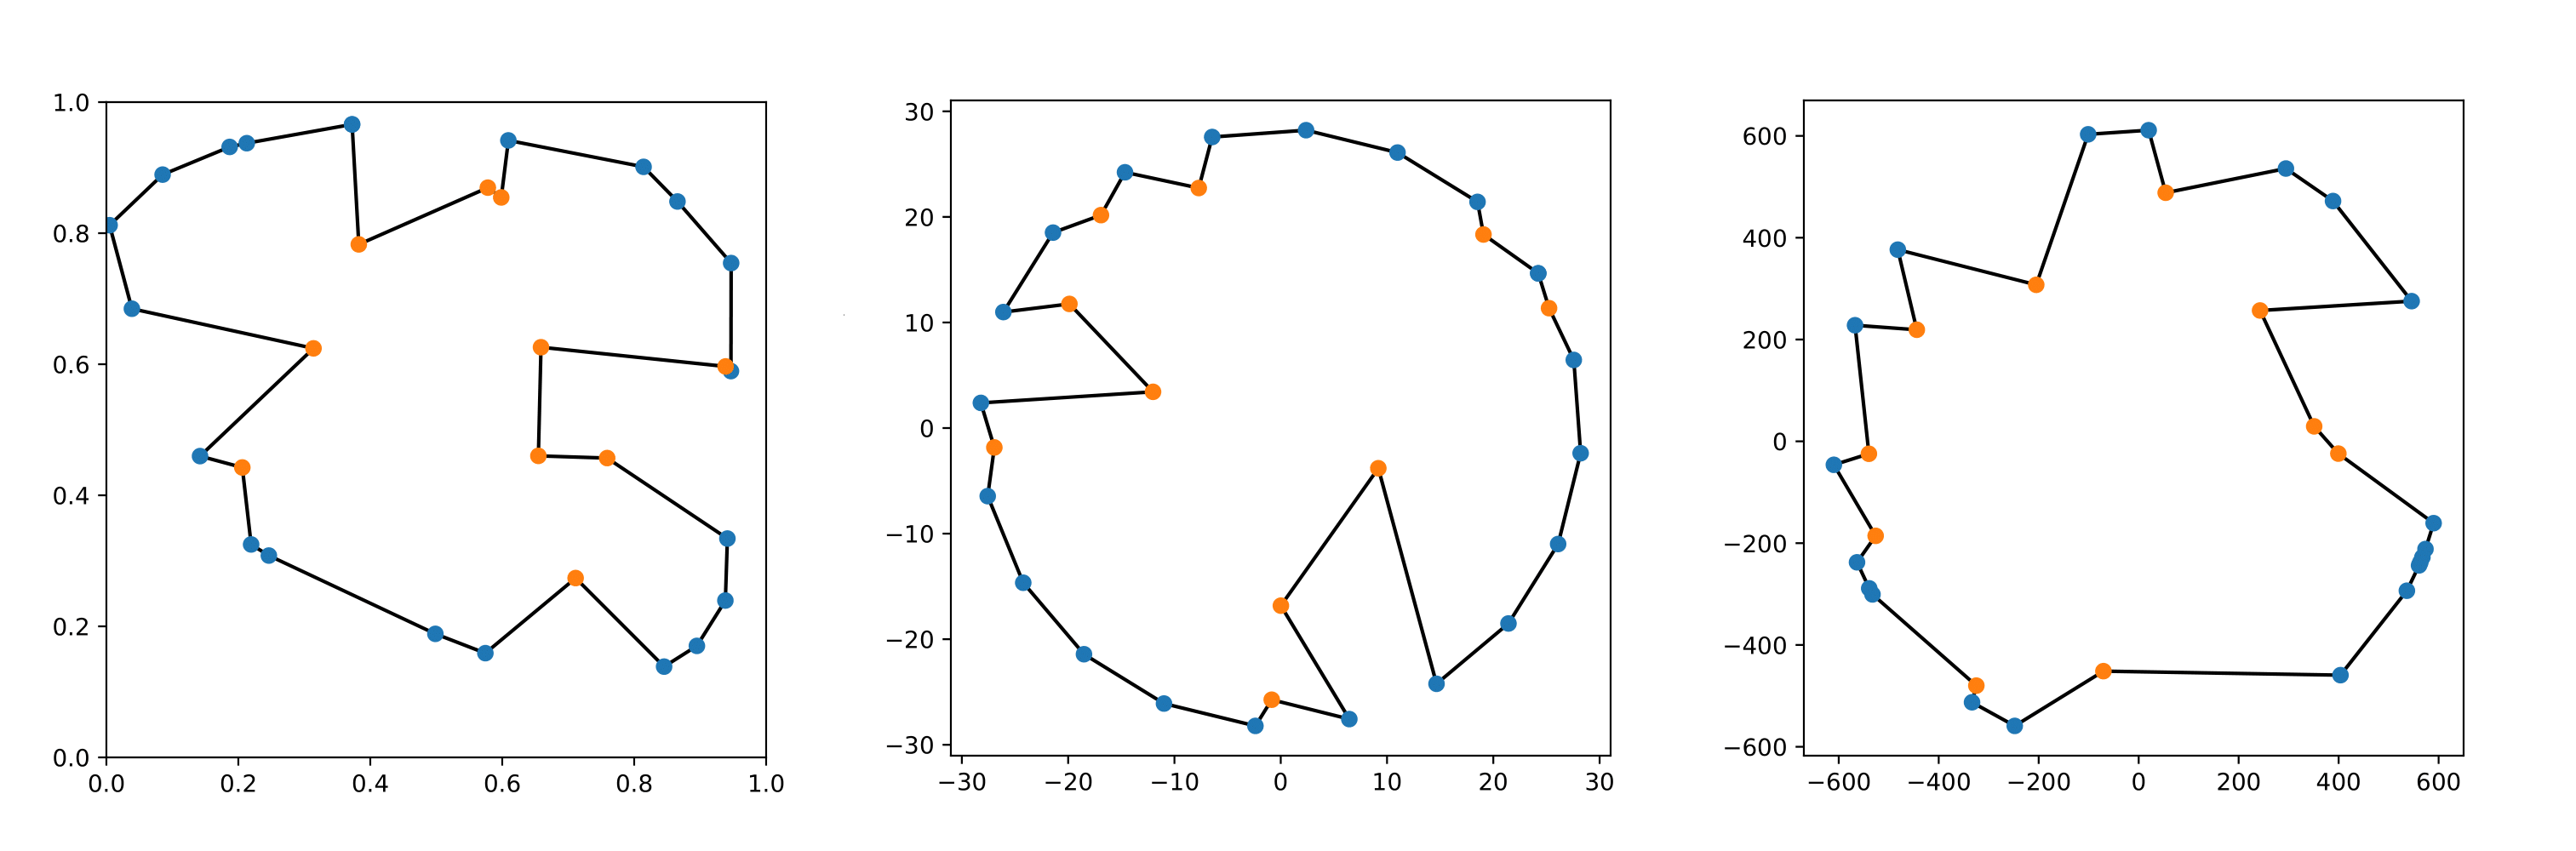
\includegraphics[width = \textwidth]{primeri_20_10.png}
    \caption{Generiranje algoritma na posameznih vrstah podatkov pri $n=20$ in $k=10$}
\end{figure}



čas trajanja algoritma pa smo zapisali v csv detoteko za vrednosti, ko je število 
zunanjih točk $10$, $20$ in $30$, za vsak $n$ pa smo izvedli $10$ ponovitev algoritma za $k$ v vrednostih od $0$ do $14$.



\section{Analiza rezultatov}
Na vsakem scenariju podatkov smo pognali algoritem tako, da nam je vrnil čas
izvajanja algoritma.  Podatke smo generirali desetkrat za vsak par argumentov,
ko je bilo število zunanjih točk $10$, $20$ in $30$, $k$ pa je zavzel vrednosti od $0$ do $14$.
Generirane rezultate smo zapisali v \emph{csv} detoteko, da smo jih lažje uvozili
v programski jezik $R$, kjer smo jih obdelali. Iz vektorja večih ponovitev za vsak par argumentov $(n,k)$, smo izračunali 
povprečje, da smo dobili čim realnejše podatke, nato pa smo za vsakega od teh vektorjev izračunali še varianco podatkov, 
da bi videli, kako različna odstopanja od povprečja dobimo za vse tri scenarije podatkov.

\begin{figure}[h!]

	\begin{subfigure}[t]{0.45\textwidth}
		\centering
		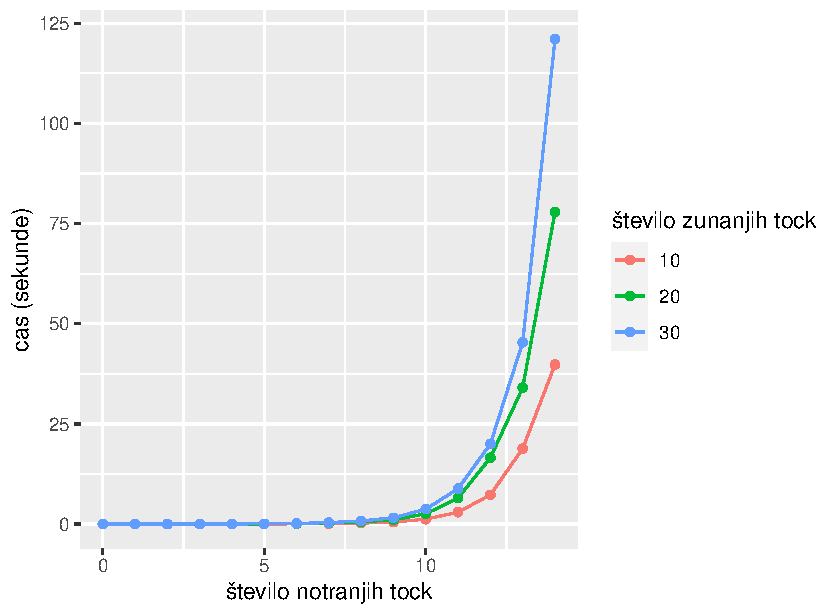
\includegraphics[width=\textwidth]{cas_izvajanja_algoritma_za_nakljucno_generiran_konveksni_poligon.pdf}
		\caption{čas izvajanja algoritma za naključni konveksni poligon}
		\label{n_10_count}
	\end{subfigure}
	\hfill
	\begin{subfigure}[t]{0.45\textwidth}
		\centering
		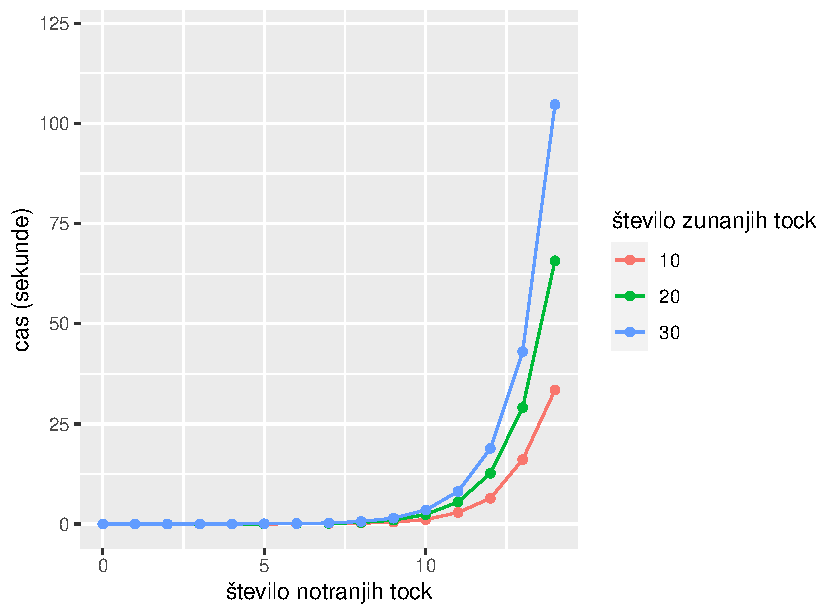
\includegraphics[width=\textwidth]{cas_izvajanja_algoritma_za_nakljucne_tocke_na_kroznici.pdf}
		\caption{čas izvajnja algoritma za naključne točke na krožnici}
		\label{n_10_time}
	\end{subfigure}
    \label{fig:n_10}
\end{figure}

Na zgornjih grafih smo prikazali, kako se z odvisnostjo od $k$ za $n\in \{10,20,30\}$ spreminja čas izvajanja algoritma,
ko zunanje točke tvorijo naključen konveksen polinom ali pa naključne točke na krožnici. Opazimo, da čas z večanjem $k$
eksponentno narašča, kar je posledica, da naš algoritem zadošča Teoremu 1 in je rešljiv v času $O(2^kk^2n)$. Zanimivo je 
še, da so časi izvajanja algoritma, ko so točke raporejene po krožnici manjše. Spodaj primerjajmo še čase vseh treh scenarijev
za $n=30$ na enem grafu.
\begin{figure}[h!]
    \centering
    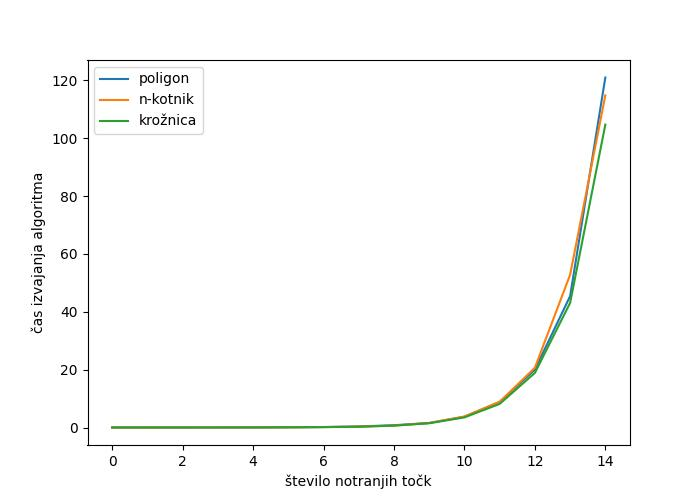
\includegraphics[width = \textwidth]{povprecje_30.jpg}
    \caption{Generiranje algoritma na posameznih vrstah podatkov pri $n=30$}
\end{figure}

Iz grafa lahko razberemo, da če so naše zunanje točke rezporejene po krožnici naključno, bo čas, ki ga algoritem
potrebuje za izračun najkrajšega obhoda, skoraj povsod manjši, kot če vzamemo katerega od ostalih dveh scenarijev.
Naključen konveksni poligon in pravilni n-kotnik se izmenjujeta na prvem mestu po porabi časa, a naši rezultati pri 
zadnji točki nakazujejo, da če bi še povečevali število notranjih točk, bi največ časa algoritem porabil za naključni
konveksni poligon, kar nam pove, da so čisto naključne razporeditve vendarle najbolj časovno potratne.\\

Za risanje zgornjih grafov smo za vsako vrednost uporabili povprečje desetih izmerkov. Zanimalo nas je, kakšno je 
odstopanje podatkov za posamezen scenarij, zato smo izračunali varianco izmerkov in jo za $n=30$ prikazali na spodnjem
grafu.

\begin{figure}[h!]
    \centering
    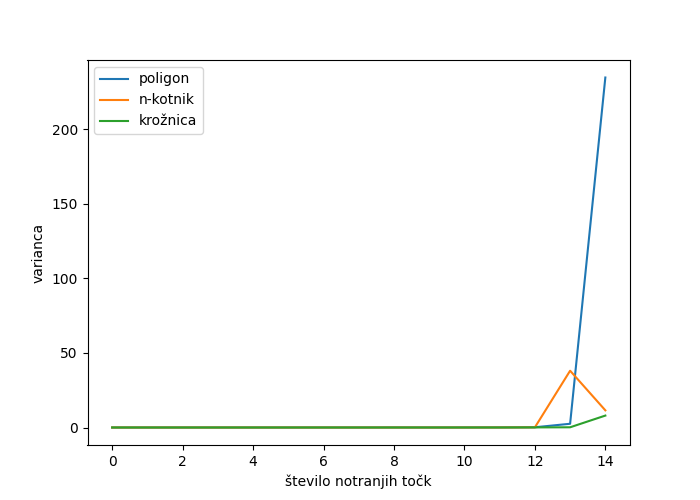
\includegraphics[width = \textwidth]{varianca.png}
    \caption{Varianca izmerkov pri posameznih scenarijih podatkov za $n=30$}
\end{figure}

Ker so na začetku časi izvajanja algoritma kratki, so tudi variance majhne, ko je $k$
manjši od $10$. Ko pa je $k=12$ postane razlika med posameznimi scenariji zelo velika.
Opazimo, da je varianca v primeru naključno izbranih točk na krožnici
najmanjša, izmerki se ves čas gibljejo okoli povprečja. Po drugi strani pa varianca
v primeru naključnega poligona skokovito naraste, razlike med izmerki so precej velike,
zato bi bilo morda potrebnih več kot le $10$ izmerkov, da bi bolj natančno določili tudi
same povprečne čase trajanj algoritma za večje $k$.

\section{Zaključek}
Po tem ko smo generirali algoritem in ga implementirali na različne podatke, smo ugotovili,
da je kot predvidevano algoritem zelo učinkovit, ko je število notranjih točk še manjše od $14$.
Ker zahtevnost eksponentno narašča, traja algoritem vedno več časa in zavzame tudi vedno več prostora.
Težave so se jasno pokazale, ko smo preizkušali algoritem in je program javil spominsko napako, še preden 
smo ga preizkusili za $20$ notranjih točk. Ugotovili smo, da algoritem daje rezultate z najmanjšo varianco 
za podatke, ki jim z dodatnimi pogoji damo še več omejitev za zunanje točke, poleg te, da morajo ležati v konveksnem
položaju.





\











\end{document}